\documentclass[pdf]{iucr}
%% \documentclass[preprint]{iucr}
\journalcode{M}

\usepackage{style}      % Custom style
%% \addtocounter{table}{0}
%% \addtocounter{figure}{-1}

% Font
% Use pdflatex to compile documents (default)
%% \usepackage{nativefont}
% Use xelatex to compile documents
%% \usepackage{xefont}

%% % Use minted to customize code highlight
%% \usepackage{minted}
%% \usemintedstyle{vs}
%% \definecolor{codebg}{HTML}{282828}

%% % Workaround to display bold font in math mode
%% % Source: https://tex.stackexchange.com/questions/565069/beamer-bold-math-no-longer-working
%% \DeclareFontShape{OT1}{cmss}{b}{n}{<->ssub * cmss/bx/n}{}

%% %---------------- show page layout. don't use in a real document!
%% \usepackage{showframe}
%% \renewcommand\ShowFrameLinethickness{0.15pt}
%% \renewcommand*\ShowFrameColor{\color{red}}

\includeonly
{
    %% sections/inbox,
    sections/introduction,
    sections/background,
    sections/model,
    sections/experiments,
    sections/conclusions,
}

\begin{document}

    % Metadata
    %FIXME (iris) suggested title
    %\title{Automating Diffraction Pattern Classification in Single-Particle Imaging Experiments with a Siamese Neural Network}
    %% \title{One-Shot Learning for Real-Time Scattering Pattern Classification in
    %% Single-Particle Imaging Experiments}
    \title{Hit classification in single-particle imaging experiments with a siamese neural network}
    \cauthor[a]{Cong}{Wang}{cwang31@stanford.edu}{}
    \author[a]{Hsing-Yin}{Chang}
    \cauthor[a]{Chun Hong}{Yoon}{yoon82@stanford.edu}{}
    \aff[a]{SLAC National Accelerator Laboratory, 2575 Sand Hill Road, Menlo Park, CA 94025, USA}

    \maketitle

    % Contents
    %% {

    I will explore model generalizability in two directions — (1) similar size,
    different shapes;  (2) different size, similar shapes (which might be harder
    to find those cases in PDB).  Accordingly, the paper about this new networks
    can also diverge into two directions: (1) A paper about application of large
    computing facilities for enabling real-time SPI classification; (2) A paper
    about a generalized model for enabling real-time SPI classification.

}

    \section{Introduction}

% (1) What is SPI and what problem in SPI have I been tackling?  
% - SPI is an important technique and where it stands in the structural biology toolkits.
%   - Room temperature.
%   - No need for crystalline.
%   - One or two sentences to show why it's important.  
% - SPI scattering patterns are like what, and classification is the problem.

Single-particle imaging (SPI) with X-ray free-electron lasers (XFELs) is a
promising method of determining the three-dimensional structure of
noncrystalline biomolecules at room temperature.   In SPI experiments,
femtosecond coherent X-ray beams strike biomolecules sprayed into the beam path,
causing scattering of radiation before destruction of the samples inflicted by
the intense X-rays.  This way of collecting scattering datasets is known as the
'diffraction before destruction' approach
\cite{neutzePotentialBiomolecularImaging2000,
chapmanFemtosecondDiffractiveImaging2006,seibertSingleMimivirusParticles2011,
aquilaLinacCoherentLight2015,reddyCoherentSoftXray2017}.  Scattering patterns in
SPI experiments largely fall into four categories, depending on how X-ray pulses
hit sample particles delivered through jet streams.  Astonishingly, 98\% X-ray
pulses miss their target particles
\cite{shiEvaluationPerformanceClassification2019}, leading to no scattering
pattern identified as a 'no hit'.  When X-ray photons collides with one and only
one sample particle, the emerging scattering pattern is defined as a 'single
hit'. Expectedly, a 'multi hit' happens when X-ray pulses and a cluster of
sample particles intersect. In some cases, X-ray pulses might hit non-biological
objects in delivery medium and those resulting scattering patterns are labeled
as 'unintended hit'.  Among the four categories, only 'single hit' images will
contribute to reconstruction of electron density maps through downstream data
processing, e.g. orientation recover and phase retrieval.  Therefore, an
efficient SPI scattering pattern classifier is long desired, but building one
has remained to be an elusive task.


% (2) The core challenges in the classification problems are this and that.
% ...Previous work on X has addressed with Y
% 
% - unsupervised method
%   - typically problem-specific
%   - prior knowledge about the location of deisred cluster needs to be known.  
% - supervised method
%   - some requires complete retraining.  
%   - requires fine tune, like the layers of the network.  
%   - still relies on hit finding for binary classifier, whereas classifier doesn't care.  

Some pioneering works that address the challenge of classifying SPI scattering
pattern have been developed.  Unsupervised methods
\cite{yoonUnsupervisedClassificationSingleparticle2011,
giannakisSymmetriesImageFormation2012,schwanderSymmetriesImageFormation2012,
yoonNovelAlgorithmsCoherent2012,
andreassonAutomatedIdentificationClassification2014,
bobkovSortingAlgorithmsSingleparticle2015a} focus on extracting features from
image samples and finding clusters of 'single hit' images.  However,
unsupervised solutions are highly problem-specific, that is to say, it's not
realistic to expect 'single hit' images from different biological samples would
form clusters that overlap in the feature space.  Moreover, despite being
unsupervised, those solutions also require prior knowledge of data distribution
in feature space for classification, rendering it incapable of being automated.
Supervised solutions based on neural network models learn from labelled images
and provide predicted classification
\cite{shiEvaluationPerformanceClassification2019,
ignatenkoClassificationDiffractionPatterns2021}.  Convolution neural networks
(CNN) were employed for feature extraction and a fully connected layer is
directly attached to the convolutional layers for classification.  Training such
networks demands a large sample size for each class, which might not be
available during the course of data collection.  Specifically, the population of
images vary substantially across different classes, resulting in imbalanced
training data detrimental to model training.  


% (3) In this work, we do this.  Concretely, our contributions are ... Siamese
% neural network.  
% Challenges:
% - Limited number of SPI images.
% - Robust against different sizes of particles.  (beat human level performance)
% - 

In this work, we strive to approach the goal of classifying scattering patterns
in nearly real-time SPI data collection {\color{gray} with a figure to summarize
what it is}.  

%% We propose a Siamese network for diffraction pattern classification.  

%% {
%% \setlength{\parindent}{4em}
%% \color{gray} 
%% 
%% \indent What is it concretely?  Embedding network, triplet loss function,
%% training strategies, validation strategies, 
%% 
%% }



% (4) This results in what appealing properties 
%     and our experiments show this and that.
% High accuracy with less training examples.  

\

Describe the unqiue characteristics of Siamese network and triplet loss
function.  Our experiments show a high accuracy for diffraction pattern
classification using this model.

    \section{Related work}

\subsection{Classifying hits from SPI images}

The task of hits classification from SPI images has been explored for over a
decade. Prior to the first CXIDB data deposition
\cite{seibertSingleMimivirusParticles2011} was available to the public, hit
classification can be performed by evaluating a cross-correlation of two SPI
images in polar coordinates \cite{bortelClassificationAveragingRandom2009}.  An
alternative classification approach was based on expectation maximization (EM)
\cite{dempsterMaximumLikelihoodIncomplete1977}, which is later integrated in EMC
method \cite{lohReconstructionAlgorithmSingleparticle2009}, a widely applied
particle reconstruction method in Cryo-EM.  Additionally, a combination of size
filtering, feature vectors and PCA was used for achieving a better single hit
classification \cite{bobkovSortingAlgorithmsSingleparticle2015}.  More recently,
artificial neural network models have become a new avenue for exploring
classification solutions with the advent of capable infrastructures (GPUs, ML
frameworks) for model training. \cite{shiEvaluationPerformanceClassification2019}
uses a CNN model  and \cite{ignatenkoClassificationDiffractionPatterns2021}
employs off-the-shell YOLO models \cite{redmonYOLO9000BetterFaster2016,
redmonYOLOv3IncrementalImprovement2018}.  Both models are trained to performance
binary classification for identifying \textit{single-hit}.  However, they use a
fully connected layer (FC) as the classifier that is directly attached to their
vision modules (CNN).  This design has been known for its inefficiency to train
as pointed out in \cite{schroffFaceNetUnifiedEmbedding2015}.  It turned out the
YOLO model in \cite{ignatenkoClassificationDiffractionPatterns2021} takes more
than three hours to train before it achieves an accuracy of 95\% in predicting
single hits.  The training time is not clear in
\cite{shiEvaluationPerformanceClassification2019}, but its accuracy is 83.8\%.
In contrast, our model demonstrates high accuracy while keeping training time
short.  


\subsection{Generalizing a classifier}

To our knowledge, there are no solution proposed to generalize a SPI hit
classifier.  However, many approaches have been developed to generalize object
recognition in computer vision.  One of the early example is signature
verification using a siamese neural network
\cite{bromleySignatureVerificationUsing1994}.  The model basically measures the
distance between two signature embeddings generated from two identical neural
networks, which learn to seperate embeddings of different signatures in a latent
space and vice versa.  The idea of siamese networks are later applied in face
recognition/verification \cite{chopraLearningSimilarityMetric2005}.  In the last
decade, another breakthrough in face recognition is demonstrated by the use of
triplet loss in \cite{kochSiameseNeuralNetworks2015a}, where both a positive
example and a negative example are constrated against an anchor example. Beyound
signature or face verification, few-shot learning problems also require
generalizing an existing classifier to identifying new categories of things not
seen by the model before.  For example, \cite{vinyalsMatchingNetworksOne2017}
introduced "matching networks" that learn to query an unlabeleed example against
one of the examples in a small support set that have new labels.
\cite{snellPrototypicalNetworksFewshot2017} proposed a prototypical network that
learns a metric space where classification is effecetively done by measuring
distances between the representation of an unlabelled example and the prototype
representation of each new class.  In our application, we choose to use triplet
loss method to train a SPI hit classifier.  In contrast to the thresholding in
FaceNet which requires tuning an additional hyperparameter, our model treats an
input image as a query item, which is then subject to similarity tests against
precomputed embeddings from each hit class.  This approach is also easy to
implement because the number of hit classes is three as opposed to faces of
incredibly many new identities in face verification problem.  


    %
    




















\section{Our model and the training strategy}

The practical goal of our model is to identify \textit{single-hit} while data
collection is still underway.  From a model perspective, we essentially use the
same neural network architecture to create an experiment-specific hit classifier
and a generalized hit classifier.  We focus more on explaining how our
experiment-specific classifier works, considering it will have an immediate
impact on real-time classification.  


\subsection{CNN vision backbone}

Our CNN vision backbone consists of two convolutional layers that extract image
features and two fully connected layers that compress these image features into
a low dimensional embedding.  The first convolutional layer uses a $5 \times 5$
single channel filter with a stride of one and no padding.  The second
convolutional layer employs a 32-channel $5 \times 5$ filter with a with a
stride of one and no padding.  A ReLU activation function is applied to the
outcome of each convolutional layer, which is followed by a max-pooling
operation performed by a $2\times 2$ filter with a stride of two.  Then, two
fully connected layer are used to generate the final embedding with the size of
128.  As a result, all SPI hits are encoded into embeddings in a latent space,
where embedding distance between two images, estimated by a squared $L2$
distance, is a measurement of their similarities.  Expectedly, identically
labeled hits should have a small embedding distance, whereas differently labeled
hits should have a large embedding distance.  

% Maybe discuss how many parameters are involved depending on the image cropping
% and downsizing in data preprocess.  

%% row x col x filters
%% \renewcommand{\arraystretch}{1.4}
%% pnCCD: 
\begin{table}
\caption{

    The architecture of the CNN vision backbone.  We only specify architectural
    parameters that are independent of input image dimensions.  The benefit is
    that those parameters can be readily used in machine learning frameworks,
    such as PyTorch or Tensorflow.  The exact value of $*$ in the layer ``FC 3"
    depends on the input image size, and can be figured out during the
    initialization of the network.  

}
%% \resizebox{1.0\textwidth}{!}{
    \begin{tabularx}{\textwidth}{   l | l l X X X  }
        Layer       &  In channels    & Out channels    & Kernel size & Stride       & Padding     \\
        \hline
        Conv 1      &  1              & 32              & 5           & 1            & 0           \\
        ReLU 1      &  \textemdash    & \textemdash     & \textemdash & \textemdash  & \textemdash \\
        MaxPool2D 1 &  \textemdash    & \textemdash     & 2           & 2            & 0           \\
        Dropout 1   &  \textemdash    & \textemdash     & \textemdash & \textemdash  & \textemdash \\
        \hline
        Conv 2      &  32             & 64              & 5           & 1            & 0           \\
        ReLU 2      &  \textemdash    & \textemdash     & \textemdash & \textemdash  & \textemdash \\
        MaxPool2D 2 &  \textemdash    & \textemdash     & 2           & 2            & 0           \\
        Dropout 2   &  \textemdash    & \textemdash     & \textemdash & \textemdash  & \textemdash \\
        \hline
        \hline
        Layer       &  In features    & Out features    & \textemdash & \textemdash  & \textemdash \\
        \hline
        FC 3        &  *              & 512             & \textemdash & \textemdash  & \textemdash \\
        ReLU 3      &  \textemdash    & \textemdash     & \textemdash & \textemdash  & \textemdash \\
        \hline
        FC 4        &  512            & 128             & \textemdash & \textemdash  & \textemdash \\
    \end{tabularx}
%% }
\end{table}


\subsection{Triplet loss function for training}

How to train the CNN vision backbone to distinguish SPI hits?  We use a strategy
adopted from FaceNet \cite{schroffFaceNetUnifiedEmbedding2015} that uses a
triplet loss function for training the vision backbone.  Each input consists of
a triplet of diffraction images, which are called an anchor $x^a$, a positive
$x^p$ and a negative $x^n$. The anchor shares the same label as the positive but
different from the negative.  Two pairs will be put into a comparison in the
model. The postive pair contains the anchor and the positive $(x^a, x^p)$,
whereas the negative pair include the anchor and the negative $(x^a, x^n)$.
During training, three identical CNNs $f$ extract features from a triplet $(x^a,
x^p, x^n)$, while another component in the model measures the squared $L2$
distance in the positive pair $\|f(x^a) - f(x^p)\|_2^2$ and the negative pair
$\|f(x^a) - f(x^n) \|_2^2$, respectively.  The objective of training our CNN $f$
is to separate the negative pair $(f(x^a), f(x^n))$ more than the the positive
pair $(f(x^a), f(x^p))$ by at least a margin of $\alpha$.  Suppose there are $N$
triplets, the objective can be stated as 

\newcommand{\isep}{\mathrel{{.}\,{.}}\nobreak}
\begin{equation} \label{eq:objective}
    \begin{array}{l}
       \|f(x_i^a) - f(x_i^p)\|_2^2 + \alpha < \|f(x_i^a) - f(x_i^n)\|_2^2, \, i = 1 \isep N
    \end{array}
\end{equation}

Meanwhile, we enforce that every embedding has a unit length of one in a
$d$-dimensional latent space, namely $f(x) \in \mathbb{R}^d$ and $\|f(x)
\|_2=1$. It means that a SPI diffraction image will be mapped to a single point
on a $d$-dimensional hypersphere with a radius of one.  We can expect
identically labeled hits will get closer over the course of training and
eventually form a cluster.  The average distance between two clusters will
ultimately be at least $\alpha$ in a squared $L2$ norm sense. The largest value
of a possible $\alpha$ is 4. Since we consider only three classes, there is
plenty of room to fit them on a hypersphere.  As a result, the value of $\alpha$
can take on many values.  FaceNet choose a very small $\alpha$ because they need
to fit millions of classes onto a hypersphere and clusters have to sit close to
one another.  

To facilite the training, the objective in Eq. (\ref{eq:objective}) is turned into the
triplet loss function in Eq. (\ref{eq:triplet_loss}).

\begin{equation} \label{eq:triplet_loss}
    \sum_{i=1}^{N} \left[ \alpha + \|f(x_i^a) - f(x_i^p)\|_2^2 - \|f(x_i^a) -
    f(x_i^n)\|_2^2 \right]_+
\end{equation}


\subsection{Selection of semi-hard triplets}

A triplet can be drawn completely randomly in three steps: (1) Randomly choose
one class;  (2) Randomly sample two examples from the chosen class;  (3)
Randomly sample one example from any class other than the chosen class.  This
method, despite being easy to implement, might not deliver fast convergence when
there are many easy triplets.  We consider three kinds of triplets that might
exist during model training: easy, semi-hard and hard shown in Fig. \ref{fig:
semi-hard}.  In an easy triplet, the negative example is already separated by
at at leats a margin of $\alpha$ than the positive example.  In a hard triplet,
the negative example is actually closer to the anchor than the positive is.  In
a semi-hard triplet, the negative example still stays more apart from the anchor
than the positive example does, but the margin is smaller than $\alpha$.  The
problem with easy triplets is that they contribute to zero in the triplet loss,
and thus the training adjusts the model weights according to other triplets. The
problem with too many hard examples is that hard examples are more likely to be
a small fraction of samples, and minimization routine will prioritize the
separation of those few hard examples from the anchor that can lead to bad local
minima.  Therefore, it's a more reasonable option to select semi-hard triplets
for training.  This strategy doesn't mean to ignore hard examples at all.
Instead, once hard examples are pulled into the semi-hard zone, minimization can
eventually pull them into the easy zone. This way allows majority of the
negative examples to stay away from the anchor by a considerable margin
$\alpha$.  From a practical standpoint, the selection of semi-hard triplets is
done at the mini-batch level, where our model randomly selects a triplet that
satisfies the following condition.  

\begin{equation}\label{eq: semi-hard condition}
    \begin{aligned}[b]
    &\|f(x_i^a) - f(x_i^p)\|_2^2 \;<\; \|f(x_i^a) - f(x_i^n)\|_2^2 \;<\;
    \|f(x_i^a) - f(x_i^p)\|_2^2 + \alpha, \\
    &i = 1 \isep N
    \end{aligned}
\end{equation}

\begin{figure} 
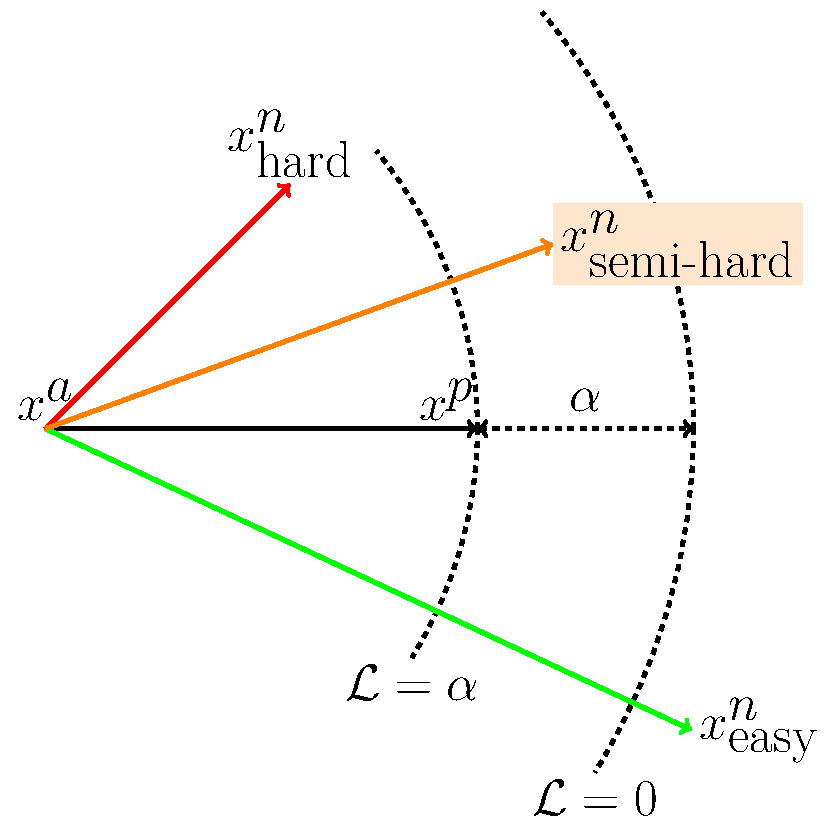
\includegraphics[width=1.0\textwidth,keepaspectratio]
{./figures/triplet.semihard.pdf} 
\caption{

    An illustration of three types of negative examples.  $x^a$ represents an
    anchor example and $x^p$ is a positive example.  Two arcs in dashed lines,
    both centered at $x^a$, are used to divide the 2D plane into three areas.
    The inner arc has a radius of $\|f(x_i^a) - f(x_i^p)\|_2^2$, whereas the
    outer arc has a radius that is larger by a margin of $\alpha$.  Negative
    examples will possess three difficult levels in model training based on the
    area where they are situated.  It's considered as a hard negative example if
    it's located within the inner arc, where $\|f(x_i^a) - f(x_i^n)\|_2^2 <
    \|f(x_i^a) - f(x_i^p) \|_2^2$.  On the contrary, it's considered as an easy
    negative example when it's goes outside the outer arc, where $\|f(x_i^a) -
    f(x_i^n)\|_2^2 - \|f(x_i^a) - f(x_i^p) \|_2^2 > \alpha$.  Lastly, it becomes
    a semi-hard negative example when it resides in the area bound between two
    arcs.  Moreover, the loss functions results in $\mathcal{L} = \alpha$ and
    $\mathcal{L} = 0$ when $x^n_{\text{semi-hard}}$ is on the inner arc and
    outer arc, respectively.  Our model training will pull
    $x^n_{\text{semi-hard}}$ close to the outer arc as much as possible, namely
    minimizing the loss.

}
\label{fig: semi-hard} 
\end{figure}


\subsection{Optimization}

%% Adam optimization algorithm

We trained our neural network models using Adam
\cite{kingmaAdamMethodStochastic2017} with the learning rate of $10^{-3}$.  The
model weights are initialized to random values from a Gaussian probability
distribution with a mean of $0.0$ and a standard deviation of $0.2$.  

\subsection{Data preprocessing}

We preprocessed SPI hit images in our application for three major reasons:
highlight features, upsample datasets and reduce image size.  Firstly, a typical
way to highlight image features is to zoom in on the region of interest (ROI) if
available.  In SPI diffraction images, features are predominantly located near
the X-ray beam center and areas remote to the center have much weaker signals.
Based on this observation, we decide to crop images by only keeping the pixels
in a user-specified ROI.  Secondly, a diffraction image collected in a SPI
experiment won't change its nature after an in-plane rotation with the beam path
as the rotational axis.  This feature allows us to upscale our dataset by
applying random in-plane rotations.  It's worth noting that any hit class, e.g.
\textit{single-hit}, can have various forms but random rotation cannot alter any
unique form of a class to resemble another one.  Lastly, we downsampled
diffraction images in our dataset by a factor of six for data collected in pnCCD
panels and two for data obtained from a simple square detector.  We don't have
an evidence to conclude those values of downsampling would always give the best
trade-off between reducing size and perserving features.  Instead, we found them
offering good enough performances through practices.  

An important caveat of upsampling our dataset is to only perform it after the
dataset is partitioned into training set and test set.  Otherwise, it will lead
to notorious ``data leakage'' issues explained in
\cite{kapoorLeakageReproducibilityCrisis2022}.  A typical consequence of ``data
leakage'' is the delusionally excellent performance of model inference during
testing, where in fact the test set already encompasses upsampled data
``leaked'' from the training set.  In another word, the ``good'' performance is
mostly caused by model memorization or overfitting.  


\subsection{Model inference}

Model inference is performed in a \textit{query-against-support} manner.  A
query is a SPI hit whose label is to be determined through inference.  In model
inference, labeled SPI hits from each class are randomly sampled to be used as
supports.  For example, when working with experimental data, we use three
support hits representing \textit{non-sample-hit}, \textit{single-hit} and
\textit{multi-hit}, respectively.  We basically label a query based on the label
of the most similar hit found in the support set.  Similarity is measured by the
squared $L2$ distance, which indicates higher similarity if its value becomes
smaller.  Fig.  \ref{fig : model inference} is an illustration of three queries,
demonstrating the labeling of a \textit{single-hit} (the first row), a
\textit{multi-hit} (the second row) and a \textit{non-sample-hit} (the third row)
.  Meanwhile, a parallel method of model inference is thresholding the distance,
which brings about an extra hyperparameter to tune.  There is no obvious winner
as whether \textit{query-against-support} is considerably better than the
threshold method.  However, when the number of unique classes is smaller, e.g.
less than four in our case, \textit{query-against-support} eliminates a
hyperparameter with a minor trade-off of sampling labeled hits to form a support
set.  We think the threshold method is a better choice when the number of unique
classes is large, e.g. $\ge 10$.  

\begin{figure}
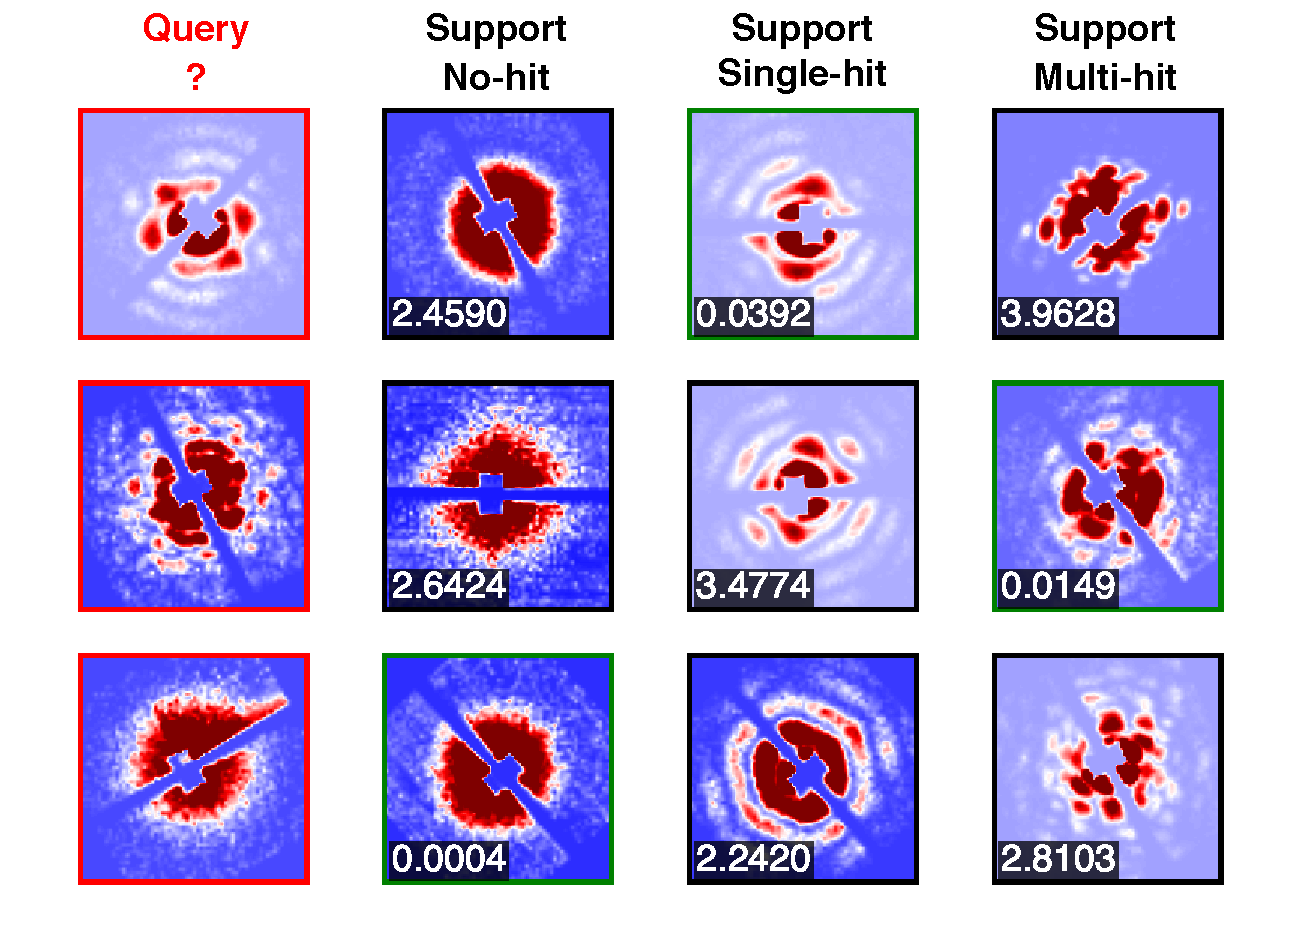
\includegraphics[width=\textwidth,height=0.8\textheight,keepaspectratio]
{./figures/inference.pdf}
\caption{

    An illustration of how the model inference is performed.  Each row
    represents a query against its support.  The predicted label for a query,
    enclosed in a red border, is inferred by the label of the most similar
    support, surrounded by a green border, in a support set, where similarity is
    measured by the squared $L2$ distance between the query and a support.
    Smaller distnace means more similar and vice versa.  

}
\label{fig : model inference}
\end{figure}

    \section{Experiments}

\subsection{Datasets}

To our knowledge, there's no existing large scale database of annotated X-ray
single particle images.  Thankfully, we can access and manually label raw
experimental data, specifically amo06516 \cite{liDiffractionDataAerosolized2020},
collected in LCLS through the Coherent X-ray Imaging Data Bank (CXIDB)
\cite{maiaCoherentXrayImaging2012}.  Meanwhile, it's challenging to
automatically scale up annotations for experimental datasets.  We then resort to
skopi \cite{peckSkopiSimulationPackage2021}, a GPU-based program for simulating
diffractive images from noncrystalline biomolecules, for concurrently
synthesizing high-resolution scatter patterns and accurate labels in an
automated manner at scale.  Lastly, we introduce three training modes that
accomodate the need in real-time classification during data collection.  

%% ImageNet
%% \cite{dengImageNetLargescaleHierarchical2009} that provides large scale
%% annotated images, .  

\subsubsection{Experimental datasets}

%% 0                : 83
%% 1                : 296
%% 2                : 177
%% 9                : 52

We chose scattering patterns from five experimental runs (90, 91, 94, 96, 102)
in the raw dataset amo06516 and categorized them into four classes: single hit,
multi hit, unintended hit and background.  It contains 296 single-hit examples,
177 double-hit examples, 83 unitended-hit example and 52 background examples.
There is a variety of variations found in the experimental dataset.  One
prominent reason is that some examples have wrong labels. Even when images are
all correctly labeled, it might still exhibit considerable variations induced by
single particle orientation, X-ray beam properties, detector configuration and
so on.  For example, a user might change detector distance from run to run, and
the scattering pattern could appear to be larger or smaller in response to the
change. Moreover, unexpected causes of variations, such as the presence of dead
pixel areas, have to be addressed on an individual basis.  



\subsubsection{Synthetic datasets}

Given any PDB file, we use skopi \cite{peckSkopiSimulationPackage2021} to
generate annotated SPI images by physically simulating scattered X-rays at a
user-specified conditions like detector distance, photon energy and so on.  We
choose to capture those simulated diffraction patterns using an artificial
simple squared detector since an artificial pnCCD detector takes up much more
storage space.  Our interest is to explore the model generalizability on
\textit{large} single particles, considering the state-of-art resolution ever
reached in an SPI experiment is still at the nanometer level ($>$ 10 $nm$)
{\color{red} (need to fact-check)} unlike in protein crystallography that
studies biological structures at the angstrom level. PDB statistics offers
direct insights on PDB data distribution by molecular weight (\url{https:
//www.rcsb.org/stats/distribution-molecular-weight-structure}).  The
example specimen, PR772 virus particles (PDB: 6Q5U),  in SPI studies, indicating that
particles with molecular weights over 380 $KDa$ can be considered as the
\textit{largest} particles.  {\color{red}(Explain on how datasets are used, more
experiments are undergoing!)} Synthetic datasets are generated by setting the
detector distance at 100.0 $mm$ and photon energy at 1.660 $keV$.  

% Insert the figure HERE and TOP..
\begin{figure}
\centering
\includegraphics[width=1.0\textwidth,keepaspectratio]{example-image}
\caption{PDB data distribution}
\label{fig:pdb_data_distribution}
\end{figure}


\subsubsection{Image mode, mosaic mode and panel mode}

One major constraint in real-time scenario is that we might not have a complete
view of a scattering pattern assembled from pixel areas of individual detector
panels.  We thus consider three different modes in dataset curation: (1) Image
mode, where information from all detector panels is consolidated according to
their respective physical locations; (2) Mosiac mode, where information from
serveral detector panels are combined without acknowleding any geometric
relations among panels;  (3) Panel mode, meaning that only pixel contents in a
single panel during a exposure is visiable to our model.  Image assembly is
trivial in offline applications, but can be complicated in real-time
applications.  Detector readouts from various panels require extra delay to
synchronize and image assembly itself might not be instantaneous, potentially
bottlenecking the FPS (frame per second) during X-ray exposure. Likewise, Mosic
mode allows the use of fewer panels, but is not able to get around the
synchronization issue either.  Conversely, panel mode is currently best suited
for real-time applications, since it doesn't have the constraints of
synchronization delay or image assembly.  One noticable limitation, though, is
that partial information about a scattering pattern on a single panel can
undermine the performance of classification.  On a side note, detectors made of
small panels might not be a good choice for high-speed SPI imaging.  


\subsubsection{Data augmentation for synthetic dataset}

% Random zooming: detect at different detector distances.

Since synthetic datasets are constructed by simulation, there are plenty for
model training on demand.  We find data augmentation still quite valuable in
providing variations caused by changes in detector distance.  For example, it is
expensive to re-simulate scattering patterns using the same particle with the
same conditions but a different detector distance.  Instead, we choose to
randomly zoom in a scattering pattern that is effectively the same as increasing
detector distance.  Zoom-out is technically more difficult to achieve for
missing pixels need to be filled in around the boarders of the original image.
We think zooming-out is not necessarily a scenario we should take into account,
as it will hurt the model performances and should be fixed from the data
collection stage, e.g. users in beamlines can adjust the detector distanecs so
that the diffraction pattern has an adequate size.  


\subsubsection{Performance on experimental data}

xxxx

\begin{figure}
\centering
\includegraphics[width=\textwidth,height=0.8\textheight,keepaspectratio]
{example-image}
\caption{Fast convergence}
\label{fig:fast_convergence}
\end{figure}

\begin{figure}
\includegraphics[width=\textwidth,height=0.8\textheight,keepaspectratio]
{example-image}
\caption{Regularization on performance}
\label{fig:regularization_on_performance}
\end{figure}


\begin{figure}
\includegraphics[width=\textwidth,height=0.8\textheight,keepaspectratio]
{example-image}
\caption{Confusion matrix (no regularization)}
\label{fig:confusion_matrix_no_reg}
\end{figure}

\begin{figure}
\includegraphics[width=\textwidth,height=0.8\textheight,keepaspectratio]
{example-image}
\caption{Confusion matrix (with regularization)}
\label{fig:confusion_matrix_with_reg}
\end{figure}

Nanorice and T4 phage

\subsubsection{Performance on synthetic data}

xxxx

\begin{figure}
\includegraphics[width=\textwidth,height=0.8\textheight,keepaspectratio]
{example-image}
\caption{PDB split vs performance}
\label{fig:confusion_matrix_with_reg}
\end{figure}

\begin{figure}
\includegraphics[width=\textwidth,height=0.8\textheight,keepaspectratio]
{example-image}
\caption{Confusion matrix (10\%)}
\label{fig:confusion_matrix_with_reg}
\end{figure}


    

















\newcommand{\RN}[1]{%
  \textup{\uppercase\expandafter{\romannumeral#1}}%
}

\section{Conclusions}

We studied the performance of triplet neural networks on identifying \textit{hit}
s in SPI experiments.  Firstly, we presented strong feasibility of applying our
model to real-time SPI \textit{hit} classification, which can be trained on a
small size dataset under 15 minutes on a moderate GPU like NVIDIA 1080 Ti.
Secondly, we also demonstrated decent generalizability of our model in
predicting \textit{single-hit}s simulated from various PDBs.  This finding
offers opportunities for building a universal \textit{hit} classifier that can
identify \textit{hit}s from distinctive biological samples.  

One major challenge of using our classifier in a real-time application is to
keep up with a potentially much higher detector readout rate.  Our model can
perform classification at a rate of nearly $450 \text{Hz}$ on a NVIDIA 1080 Ti,
which still falls far short to the $1 \text{MHz}$ detector readout rate in
facilities like LCLS-\RN{2} by three orders of magnitude.  Therefore, we propose
to incorporate \textit{hit}-filtering by intensity thresholding as the first
step, which can quickly eliminate the vast majority of ``missed-target'' shots.
Then, we follow up the \textit{hit} classification with our neural network based
classifier.  


    % Bibliography
    \bibliographystyle{iucr}
    \bibliography{bibliography}

\end{document}
